\documentclass[11pt]{article}

\usepackage[margin=1in]{geometry}
\usepackage{amsmath,amssymb}
\usepackage{graphicx}
\usepackage{booktabs}
\usepackage{array}
\usepackage{longtable}
\usepackage{caption}
\usepackage{subcaption}
\usepackage{natbib}
\usepackage{xcolor}
\usepackage{microtype}
\usepackage{hyperref}

\hypersetup{
    colorlinks=true,
    linkcolor=blue!50!black,
    citecolor=blue!50!black,
    urlcolor=blue!50!black
}

\graphicspath{{./}{../}}

\title{Controlled Organizational Memory in Spontaneous Neural Population Dynamics:\\
A Reduced HRSM State-Space Analysis of Allen Neuropixels Data}

\author{Stephen Atalebe\\
\emph{Affiliation to be confirmed}}

\date{\today}

\begin{document}

\maketitle

\begin{abstract}
Spontaneous neural activity is often treated either as background variability or as an internally structured dynamical process. This study asks whether spontaneous neural population states contain a retained historical component that improves prediction of future population organization. Allen Visual Coding Neuropixels spontaneous activity from three sessions was analyzed using a reduced homeostatic state-space model with four orthogonalized coordinates: \(H\), \(R\), \(S\), and \(M\). For each session, population activity was binned, projected into HRSM state space, and tested using aligned lag-history predictors against shuffled-lag controls. Across sessions, aligned recent history improved prediction relative to shuffled lag history. The strongest raw controlled targets were active-unit fraction and population-rate entropy, while population-state speed was weakest. Variance and autocorrelation audits narrowed the interpretation: entropy remained comparatively robust after residualization, whereas active-unit recruitment was partly variance-linked. Lag-ablation tests supported the historical nature of the effect, with recruitment and entropy remaining positive across lag sets. A descriptive ripeness index separated structural HRSM potential from memory-bearing organizational dynamics. These results support a bounded conclusion: spontaneous neural population activity contains controlled organizational memory, most visible in recruitment and entropy, without implying consciousness or a complete theory of neural dynamics.
\end{abstract}

\noindent\textbf{Keywords:} spontaneous neural activity; Neuropixels; Allen Brain Observatory; population dynamics; non-Markovian memory; entropy; recruitment; HRSM; state-space analysis.

\section{Introduction}

Neural population activity is commonly represented as an instantaneous state vector. Such a representation is necessary, but it may be incomplete. If two neural populations occupy similar current states while differing in recent history, their future organization may still diverge. The present work asks whether such reduced-state incompleteness can be detected operationally in spontaneous neural activity. The test is not philosophical. It is statistical: does aligned recent population history improve prediction of future population organization relative to a present-state baseline and relative to a shuffled-lag null?

Spontaneous neural activity is not empty baseline. Large-scale recordings have shown that spontaneous activity can be high-dimensional, structured, and related to ongoing behavior or internal state \citep{Stringer2019Spontaneous}. More recent work on latent neural states has emphasized that neural variability is shaped by non-stationary internal dynamics, behavior, and stimulus context \citep{Akella2025LatentStates}. Hidden-state analyses of spontaneous spiking activity similarly indicate that ongoing population activity can be organized into latent dynamical regimes \citep{Sederberg2024LatentDynamics}. The present study is aligned with this literature, but it focuses on a narrower question: whether retained recent history contributes to prediction of future spontaneous population organization.

The analysis uses the Allen Visual Coding Neuropixels dataset, which surveys spiking activity across cortical, thalamic, hippocampal, and related visual-system structures using high-density Neuropixels probes \citep{Jun2017Neuropixels,Siegle2021VisualHierarchy}. The Allen Brain Observatory provides standardized, reusable neurophysiology datasets and has become an important resource for computational analyses of visual coding and neural population dynamics \citep{DeVries2023AllenLessons,Xie2023VisualCodingAssessment}. Here, the stimulus-driven components of the dataset are not the primary focus. Instead, spontaneous intervals are used to test whether ongoing population dynamics carry controlled historical structure.

A reduced HRSM state-space projection is used to describe population states. HRSM refers to four operational coordinates: reserve-like population depth \(H\), recoverability-like return structure \(R\), coherence or stability \(S\), and retained-history structure \(M\). These coordinates are not treated as anatomical entities. They are data-derived summary axes designed to compress population organization into an interpretable vector space. The coordinates are orthogonalized before analysis so that subsequent memory tests are not dominated by axis redundancy.

The central memory test compares an aligned lag-history model against a baseline model and against shuffled-lag controls. The shuffled-lag null preserves lag-feature distributions while breaking temporal alignment. This distinction is essential. A positive raw memory gain may arise from target variance, autocorrelation, or model flexibility. A controlled memory gain requires that the temporally aligned past outperform a temporally disrupted past. In this work, the main statistic is therefore the observed memory gain minus the mean shuffled-lag gain.

The contribution of this manuscript is a bounded empirical result. Across three spontaneous-focused Allen Neuropixels sessions, aligned recent history improves prediction relative to shuffled-lag controls. The strongest raw controlled targets are active-unit fraction and population-rate entropy, indicating that the retained-history signal is organizational rather than simply rate-based. Robustness analyses narrow the claim: active-unit recruitment is partly entangled with variance and autocorrelation structure, while entropy survives residualization more cleanly. Lag-ablation tests support the historical character of the signal, and a descriptive ripeness index separates structural HRSM potential from memory-carrying organization.

\section{Data and preprocessing}

\subsection{Allen Neuropixels sessions}

Three Allen Visual Coding Neuropixels sessions were analyzed:
\[
715093703,\quad 719161530,\quad 750749662.
\]
For each session, spontaneous intervals were extracted for four target regions:
\[
\mathrm{VISp},\quad \mathrm{VISl},\quad \mathrm{LGd},\quad \mathrm{CA1}.
\]
Each spontaneous-focused extraction used 20 units per region, 15 spontaneous presentations, 0.25 second bins, and a maximum of 60 seconds per spontaneous presentation. Each session therefore contributed 80 selected units and 8,464 region-specific population-state rows.

The analysis used direct HDF5 access to cached NWB files rather than constructing full PyNWB session objects. This was a computational choice intended to reduce memory pressure while preserving access to spike times, unit identifiers, electrode-region metadata, and spontaneous-presentation intervals.

\subsection{Population-state matrix}

For each session and region, binned spike counts were converted into a population-state matrix. Each row represented a time-bin population state within a spontaneous presentation. The main target variables were:
\[
\texttt{population\_mean\_rate\_hz},
\]
\[
\texttt{population\_std\_rate\_hz},
\]
\[
\texttt{active\_unit\_fraction},
\]
\[
\texttt{population\_l2\_rate\_norm},
\]
\[
\texttt{population\_rate\_entropy},
\]
and
\[
\texttt{population\_state\_speed}.
\]
Active-unit fraction quantifies recruitment, while population-rate entropy quantifies the distributional organization of population activity. Population-state speed measures deformation between successive population states.

\begin{table}[t]
\centering
\caption{Spontaneous-focused extraction summary. Each session used 20 units per region, 15 spontaneous presentations, 0.25 second bins, and four regions: VISp, VISl, LGd, and CA1.}
\label{tab:extraction-summary}
\begin{tabular}{lrrrr}
\toprule
Session & Selected units & Presentations & Population-state rows & Regions \\
\midrule
715093703 & 80 & 15 & 8464 & 4 \\
719161530 & 80 & 15 & 8464 & 4 \\
750749662 & 80 & 15 & 8464 & 4 \\
\bottomrule
\end{tabular}
\end{table}

\section{HRSM state-space projection}

\subsection{Operational coordinates}

Each population state was projected into a reduced HRSM vector:
\[
\mathbf{x}_{t} = (H_t, R_t, S_t, M_t).
\]
The coordinate \(H\) represents reserve-like organized population depth. The coordinate \(R\) represents recoverability-like return structure. The coordinate \(S\) represents coherence or stability. The coordinate \(M\) represents retained-history structure. These coordinates should be read as operational state-space variables, not as direct physiological primitives.

A descriptive neural potential, denoted \(\Phi_{\rm neural}\), was computed from the HRSM coordinates to summarize state position. This quantity is not a measure of consciousness, awareness, or subjective state. It is a compact descriptor of HRSM state potential.

\subsection{Orthogonalization}

The raw HRSM proxy coordinates were orthogonalized to reduce axis redundancy. Orthogonality was audited by computing the maximum absolute off-diagonal correlation among the orthogonalized axes. Across the three spontaneous sessions, the maximum off-diagonal correlations were on the order of \(10^{-15}\), indicating numerical axis separation.

\begin{table}[t]
\centering
\caption{Cross-session HRSM and memory summary. The third session weakens two broad claims: raw memory gain is not positive in every region, and LGd is not always the highest-\(\Phi_{\rm neural}\) region. The controlled shuffled-lag result survives.}
\label{tab:session-summary}
\begin{tabular}{lrrrrl}
\toprule
Session & Best \(\Phi\) region & Best \(\Phi\) & Median gain & Median controlled gain & Top target \\
\midrule
715093703 & LGd & 0.408474 & 0.035902 & 0.039595 & active-unit fraction \\
719161530 & LGd & 0.702594 & 0.037543 & 0.041368 & active-unit fraction \\
750749662 & CA1 & 0.417804 & 0.030390 & 0.033282 & entropy \\
\bottomrule
\end{tabular}
\end{table}

\section{Memory model and shuffled-lag control}

\subsection{Aligned lag-history model}

For each target \(y_t\), a baseline model was compared against a memory model containing aligned lag-history features. The main model used lags \((1,2)\). Additional ablation models used lag sets \((1)\), \((2)\), \((1,2)\), \((1,2,3)\), and \((1,2,3,4)\). Ridge regression was used in the main audits.

Raw memory gain was defined as:
\[
\Delta R^2_{\rm raw}
=
R^2_{\rm memory}
-
R^2_{\rm baseline}.
\]

\subsection{Shuffled-lag control}

To distinguish aligned historical contribution from distributional lag-feature effects, shuffled-lag controls were generated. These controls preserved the marginal lag-feature structure but disrupted temporal alignment. Controlled memory gain was defined as:
\[
\Delta R^2_{\rm controlled}
=
\Delta R^2_{\rm observed}
-
\mathbb{E}\left[\Delta R^2_{\rm shuffled}\right].
\]
This statistic is the primary memory quantity in the manuscript.

\section{Results}

\subsection{Spontaneous HRSM states are reproducibly projected across sessions}

All three sessions produced the same extraction scale: 8,464 population-state rows per session across four regions. Orthogonalization succeeded in all sessions, with maximum absolute off-diagonal HRSM correlations of \(3.99 \times 10^{-15}\), \(4.18 \times 10^{-15}\), and \(6.14 \times 10^{-15}\). The state-space projection is therefore numerically stable at the scale used here.

The highest-\(\Phi_{\rm neural}\) state varied across sessions. LGd was highest in sessions 715093703 and 719161530, while CA1 was highest in session 750749662. This variation is important because it prevents a simple LGd-dominance interpretation. LGd remains structurally strong, but the strongest HRSM state is not fixed across sessions.

\begin{figure}[t]
\centering
\fbox{
\begin{minipage}{0.92\linewidth}
\centering
\textbf{Pipeline schematic}\\[0.5em]
Allen Visual Coding Neuropixels NWB\\
\(\Downarrow\) direct low-memory HDF5 extraction\\
Binned spike table\\
\(\Downarrow\) region-wise population-state matrix\\
HRSM projection: \(H,R,S,M,\Phi_{\rm neural}\)\\
\(\Downarrow\) aligned lag-history prediction\\
Shuffled-lag null\\
\(\Downarrow\) target sweep, variance scaling, lag ablation, ripeness
\end{minipage}
}
\caption{Analysis pipeline. Direct NWB/HDF5 extraction was used to avoid full session-object loading. Population-state matrices were projected into HRSM state space and tested using aligned lag-history models against shuffled-lag controls.}
\label{fig:pipeline}
\end{figure}

\subsection{Aligned history exceeds shuffled-lag controls across sessions}

The core memory result survives across all three sessions. The first two sessions showed positive raw mean-rate memory gain in all four regions. The third session contained one exception: VISp had a slightly negative raw mean-rate memory gain. However, the stronger controlled statistic remained positive at the session level, and every session showed observed gains above shuffled-lag means.

The session-level median observed-minus-shuffled gains were:
\[
0.039595,\quad 0.041368,\quad 0.033282.
\]
Thus, aligned recent history consistently outperformed temporally disrupted lag history.

\begin{figure}[t]
\centering
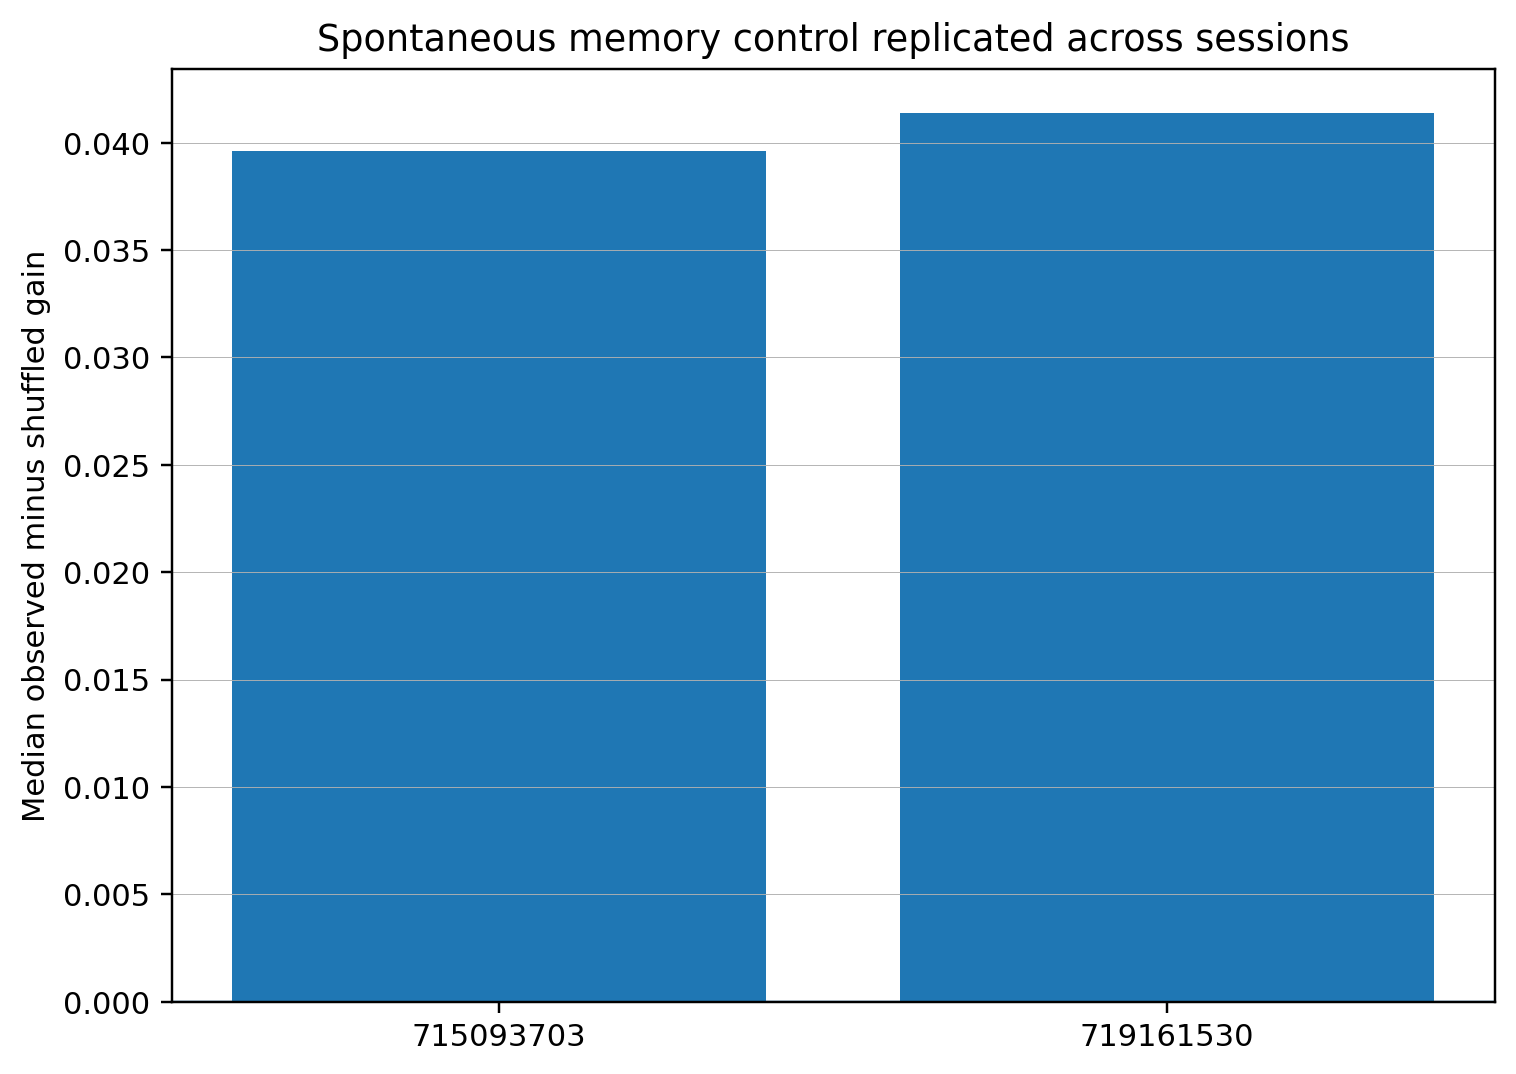
\includegraphics[width=0.75\linewidth]{results/figures/cross_session/allen_spontaneous_v1/cross_session_spontaneous_memory_control.png}
\caption{Session-level controlled memory effect. Median observed-minus-shuffled memory gain remains positive across all three spontaneous-focused Allen sessions.}
\label{fig:session-memory-control}
\end{figure}

\begin{figure}[t]
\centering
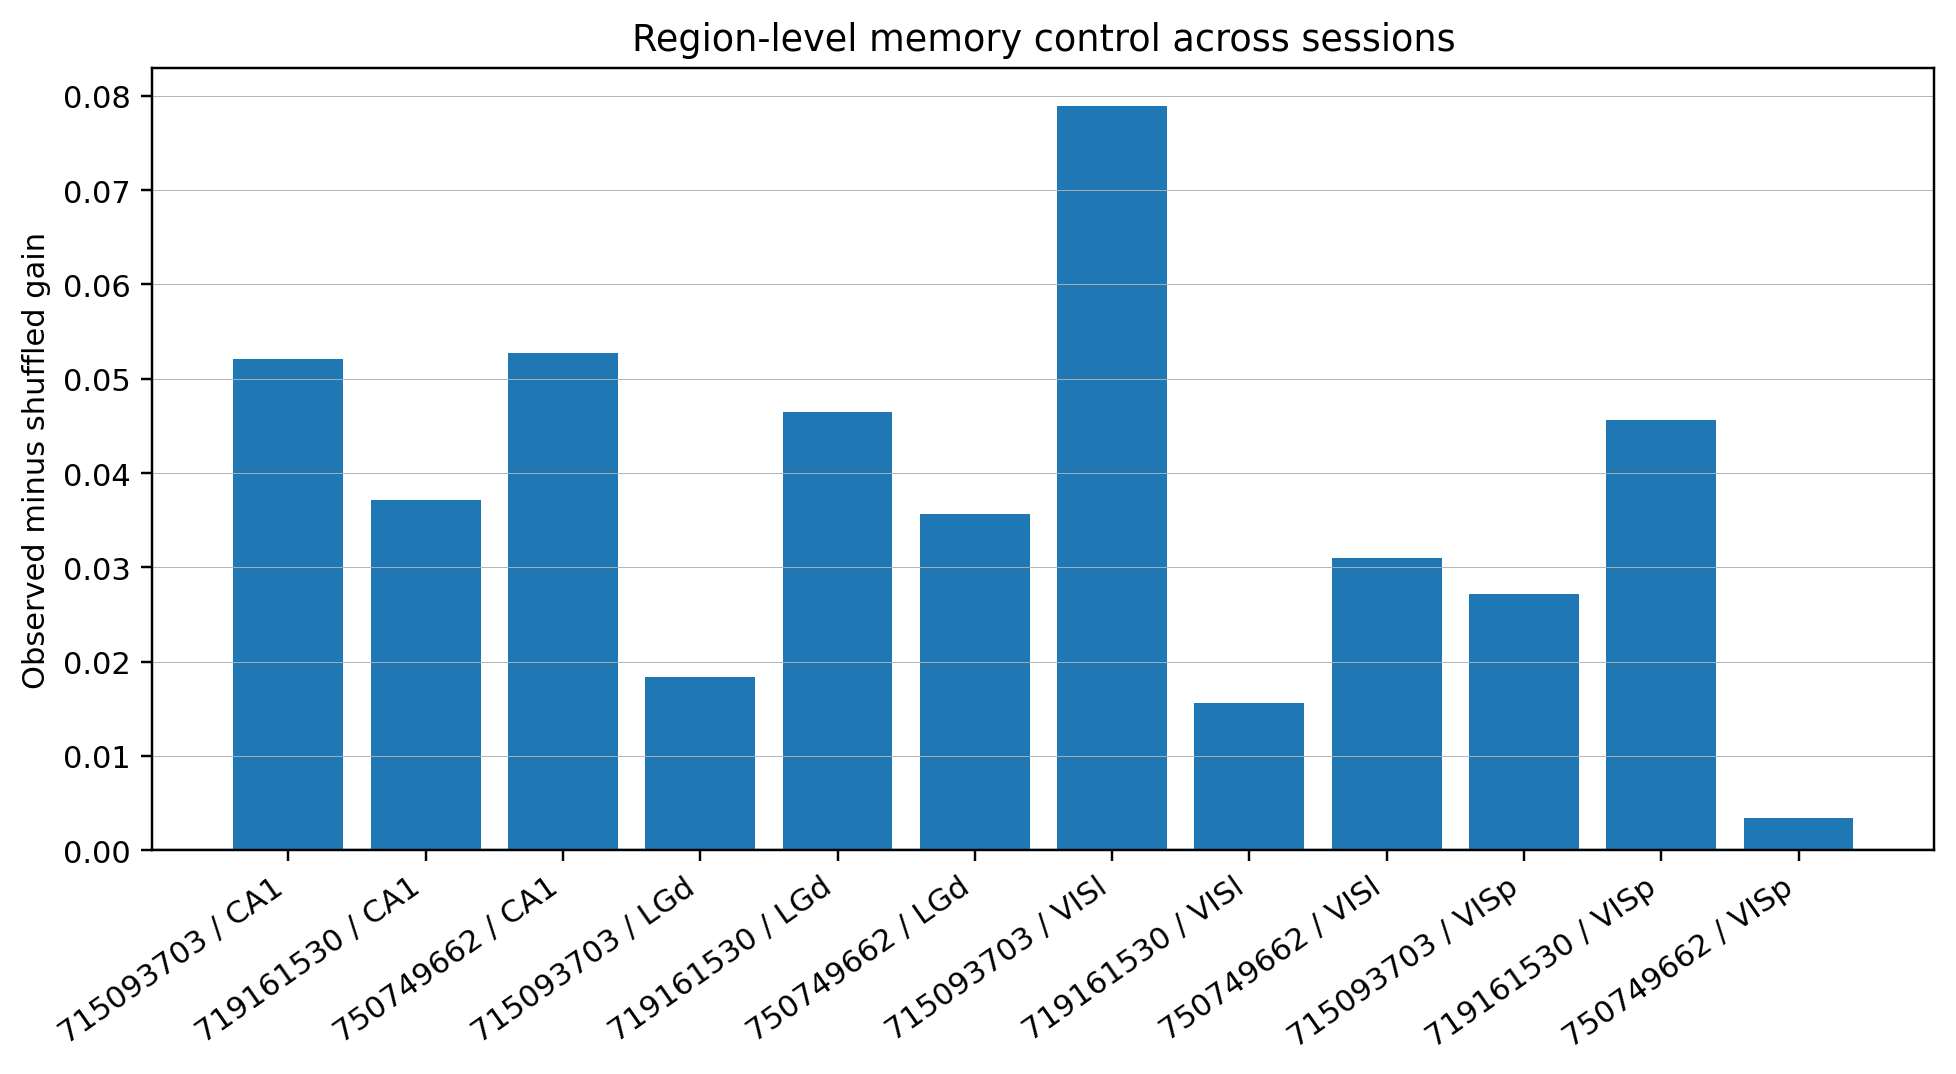
\includegraphics[width=0.85\linewidth]{results/figures/cross_session/allen_spontaneous_v1/cross_session_region_memory_control.png}
\caption{Region-level controlled memory effect. Region-level observed-minus-shuffled memory gain is positive across the analyzed spontaneous session-region states, even though raw gain is not uniformly positive in every case.}
\label{fig:region-memory-control}
\end{figure}

\subsection{Controlled memory is strongest for organizational targets}

The target sweep shows that the memory signal is not primarily a generic firing-rate effect. Across sessions, active-unit fraction and population-rate entropy are the strongest raw controlled targets. Mean firing rate ranks third, while population-state speed ranks last.

\begin{table}[t]
\centering
\caption{Cross-session target synthesis. Controlled memory is strongest for active-unit fraction and population-rate entropy.}
\label{tab:target-synthesis}
\begin{tabular}{lrrrr}
\toprule
Target & Median gain & Median controlled gain & Minimum fraction above shuffle & Rank \\
\midrule
active\_unit\_fraction & 0.062644 & 0.066169 & 1.00 & 1 \\
population\_rate\_entropy & 0.060345 & 0.064422 & 1.00 & 2 \\
population\_mean\_rate\_hz & 0.035902 & 0.039490 & 1.00 & 3 \\
population\_l2\_rate\_norm & 0.033038 & 0.036627 & 0.75 & 4 \\
population\_std\_rate\_hz & 0.024394 & 0.028737 & 0.75 & 5 \\
population\_state\_speed & 0.007906 & 0.012882 & 0.25 & 6 \\
\bottomrule
\end{tabular}
\end{table}

\begin{figure}[t]
\centering
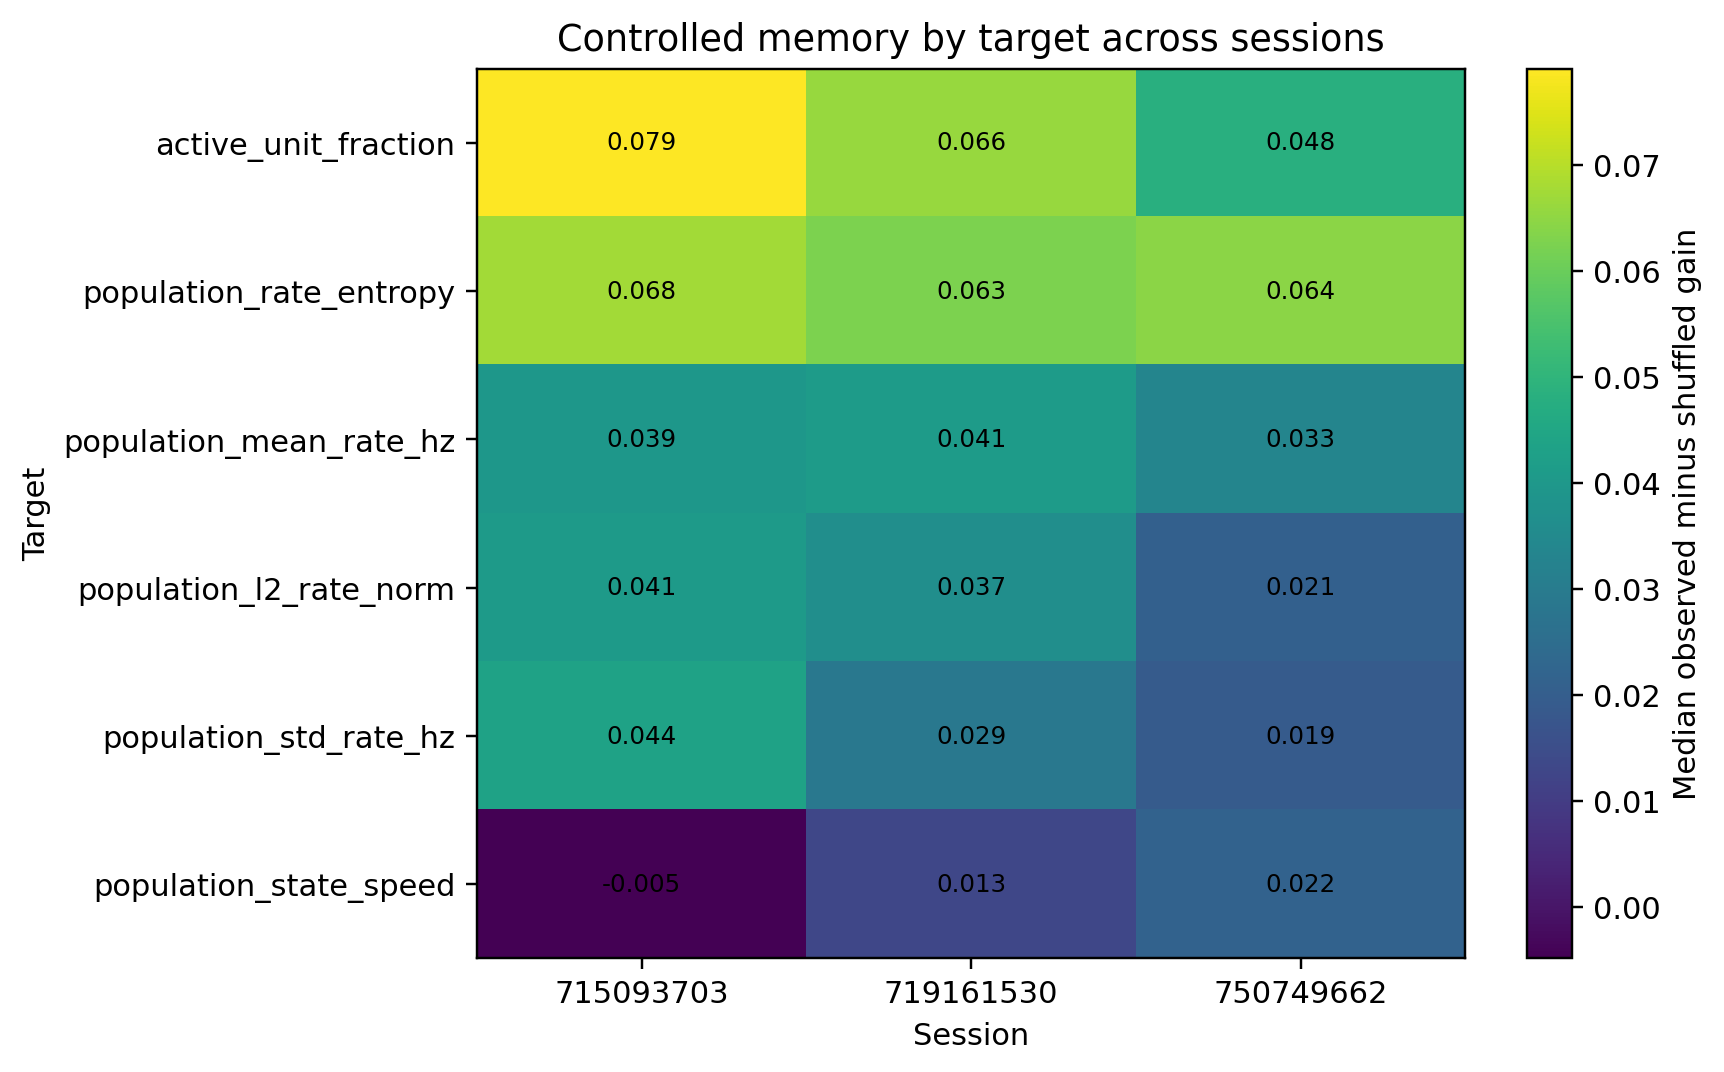
\includegraphics[width=0.85\linewidth]{results/figures/cross_session/allen_spontaneous_v1/cross_session_target_memory_heatmap.png}
\caption{Target-level controlled memory across sessions. Active-unit fraction and population-rate entropy are the strongest raw controlled targets across the spontaneous-focused sessions.}
\label{fig:target-heatmap}
\end{figure}

This target ordering motivates the phrase \emph{controlled organizational memory}. The retained historical component is most visible in variables describing participation and distributional organization, rather than in state velocity.

\subsection{Variance scaling narrows the recruitment claim}

A variance-scaling audit tested whether controlled memory gain merely tracked target variance, dispersion, or lag-1 autocorrelation. The raw controlled ranking remained led by active-unit fraction and entropy. However, after residualizing variance, lag-1 autocorrelation, and row count, active-unit fraction dropped behind population L2 rate norm and entropy. Entropy remained near the top.

\begin{table}[t]
\centering
\caption{Variance and autocorrelation residualization. Active-unit fraction leads the raw controlled ranking but is weakened by residualization. Entropy remains more stable under the residualized audit.}
\label{tab:variance-scaling}
\begin{tabular}{lrrrr}
\toprule
Target & Raw controlled gain & Raw rank & Residual gain & Residual rank \\
\midrule
active\_unit\_fraction & 0.063814 & 1 & 0.001711 & 3 \\
population\_rate\_entropy & 0.062511 & 2 & 0.007370 & 2 \\
population\_mean\_rate\_hz & 0.036210 & 3 & -0.009043 & 5 \\
population\_std\_rate\_hz & 0.033441 & 4 & -0.009630 & 6 \\
population\_l2\_rate\_norm & 0.033028 & 5 & 0.011099 & 1 \\
population\_state\_speed & 0.012205 & 6 & -0.002276 & 4 \\
\bottomrule
\end{tabular}
\end{table}

\begin{figure}[t]
\centering
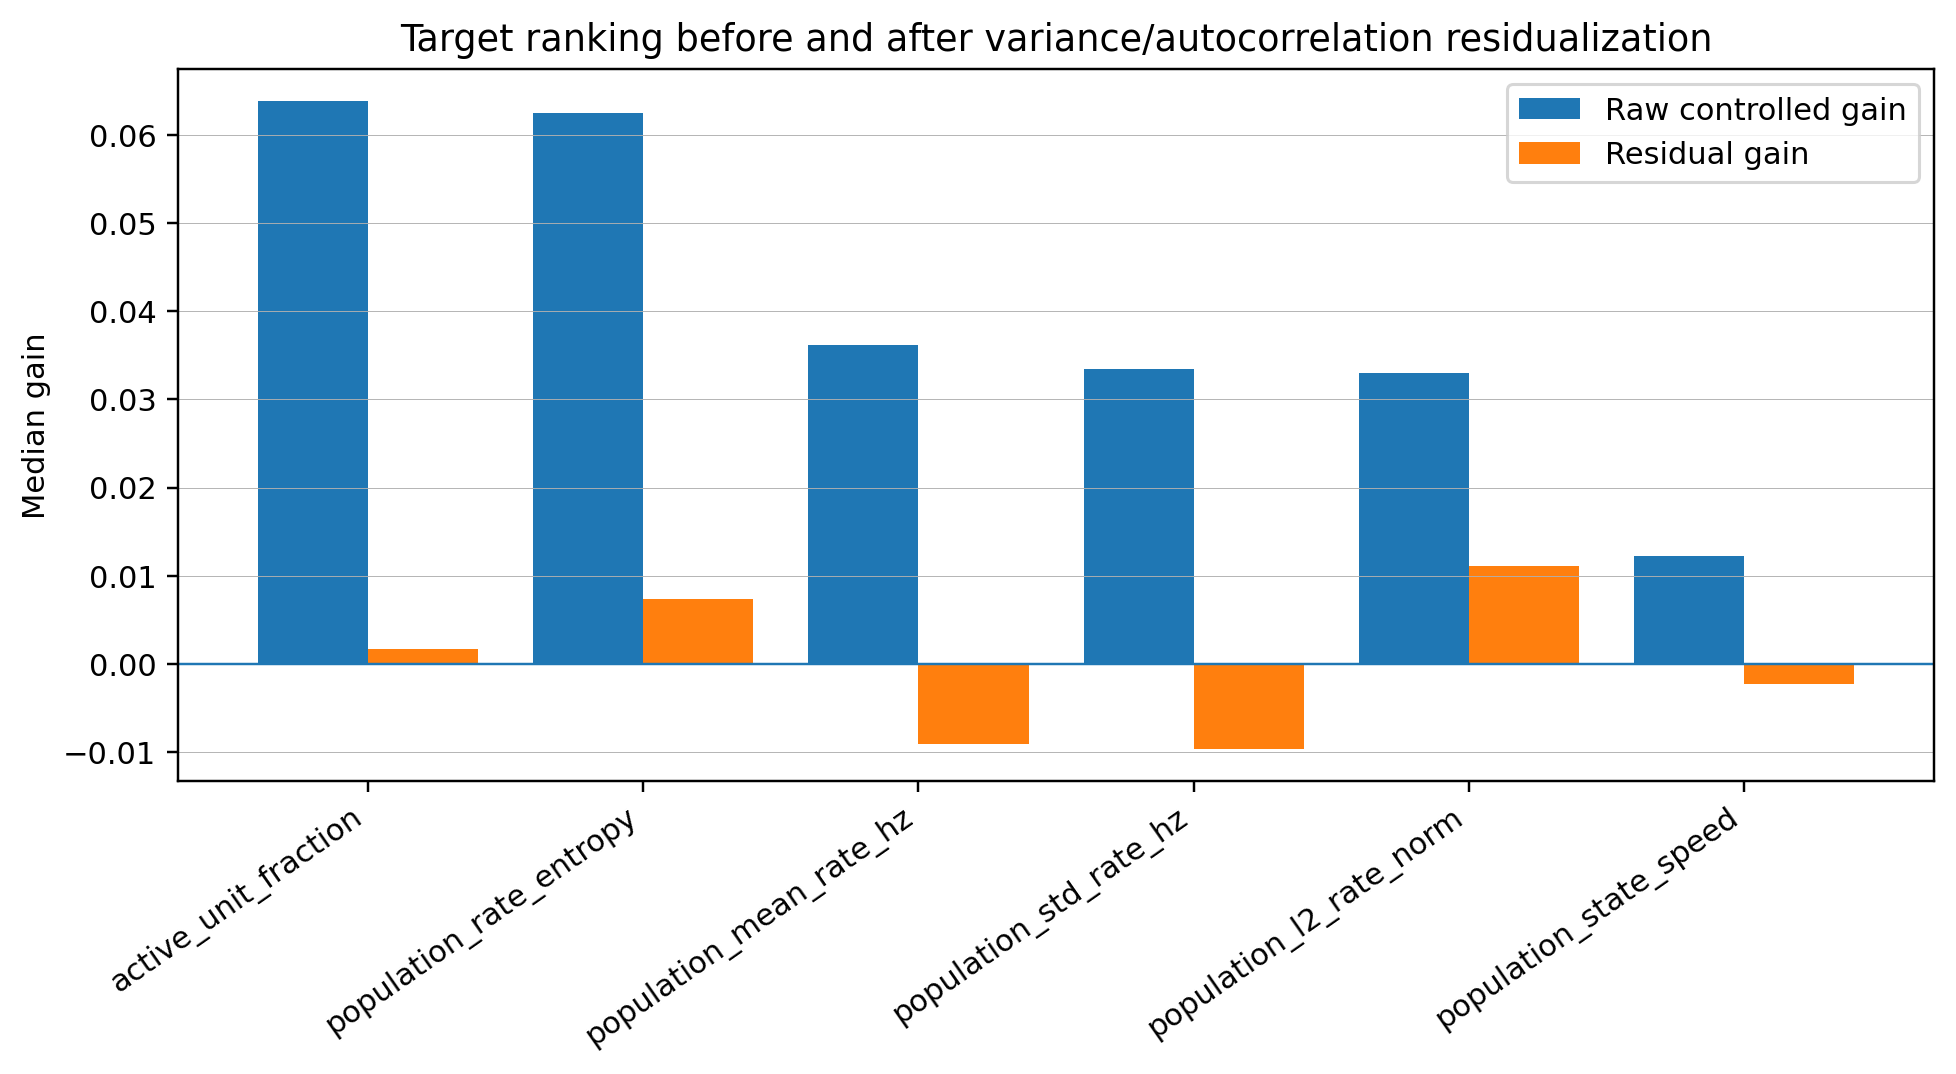
\includegraphics[width=0.85\linewidth]{results/figures/cross_session/allen_spontaneous_v1/cross_session_variance_residual_target_rank.png}
\caption{Target ranking before and after variance/autocorrelation residualization. The recruitment effect is partly entangled with target variance and autocorrelation structure, while entropy remains comparatively robust.}
\label{fig:variance-residual}
\end{figure}

The overall Spearman correlation between target variance and controlled gain was \(-0.559\), which is not negligible but does not collapse the result into a simple variance-scaling artifact. The correct interpretation is narrower: active-unit recruitment is a strong raw controlled target, but entropy is the cleaner organizational-memory target after variance/autocorrelation adjustment.

\subsection{Lag ablation supports a historical contribution}

Lag-ablation tests were run across five lag sets: \((1)\), \((2)\), \((1,2)\), \((1,2,3)\), and \((1,2,3,4)\). Active-unit fraction and entropy remained positive across all tested lag choices. The canonical \((1,2)\) lag set retained active-unit fraction and entropy as the top two targets. The controlled gains generally increased with additional recent lags.

\begin{table}[t]
\centering
\caption{Lag-ablation controlled gains. Values are cross-session median observed-minus-shuffled gains.}
\label{tab:lag-ablation}
\begin{tabular}{lrrrrr}
\toprule
Target & lag1 & lag2 & lag12 & lag123 & lag1234 \\
\midrule
active\_unit\_fraction & 0.046499 & 0.046029 & 0.066097 & 0.076122 & 0.087106 \\
population\_rate\_entropy & 0.039511 & 0.048006 & 0.064305 & 0.077218 & 0.081646 \\
population\_mean\_rate\_hz & 0.030403 & 0.027874 & 0.039064 & 0.046647 & 0.050860 \\
population\_state\_speed & 0.004257 & 0.012048 & 0.012949 & 0.012580 & 0.012323 \\
\bottomrule
\end{tabular}
\end{table}

\begin{figure}[t]
\centering
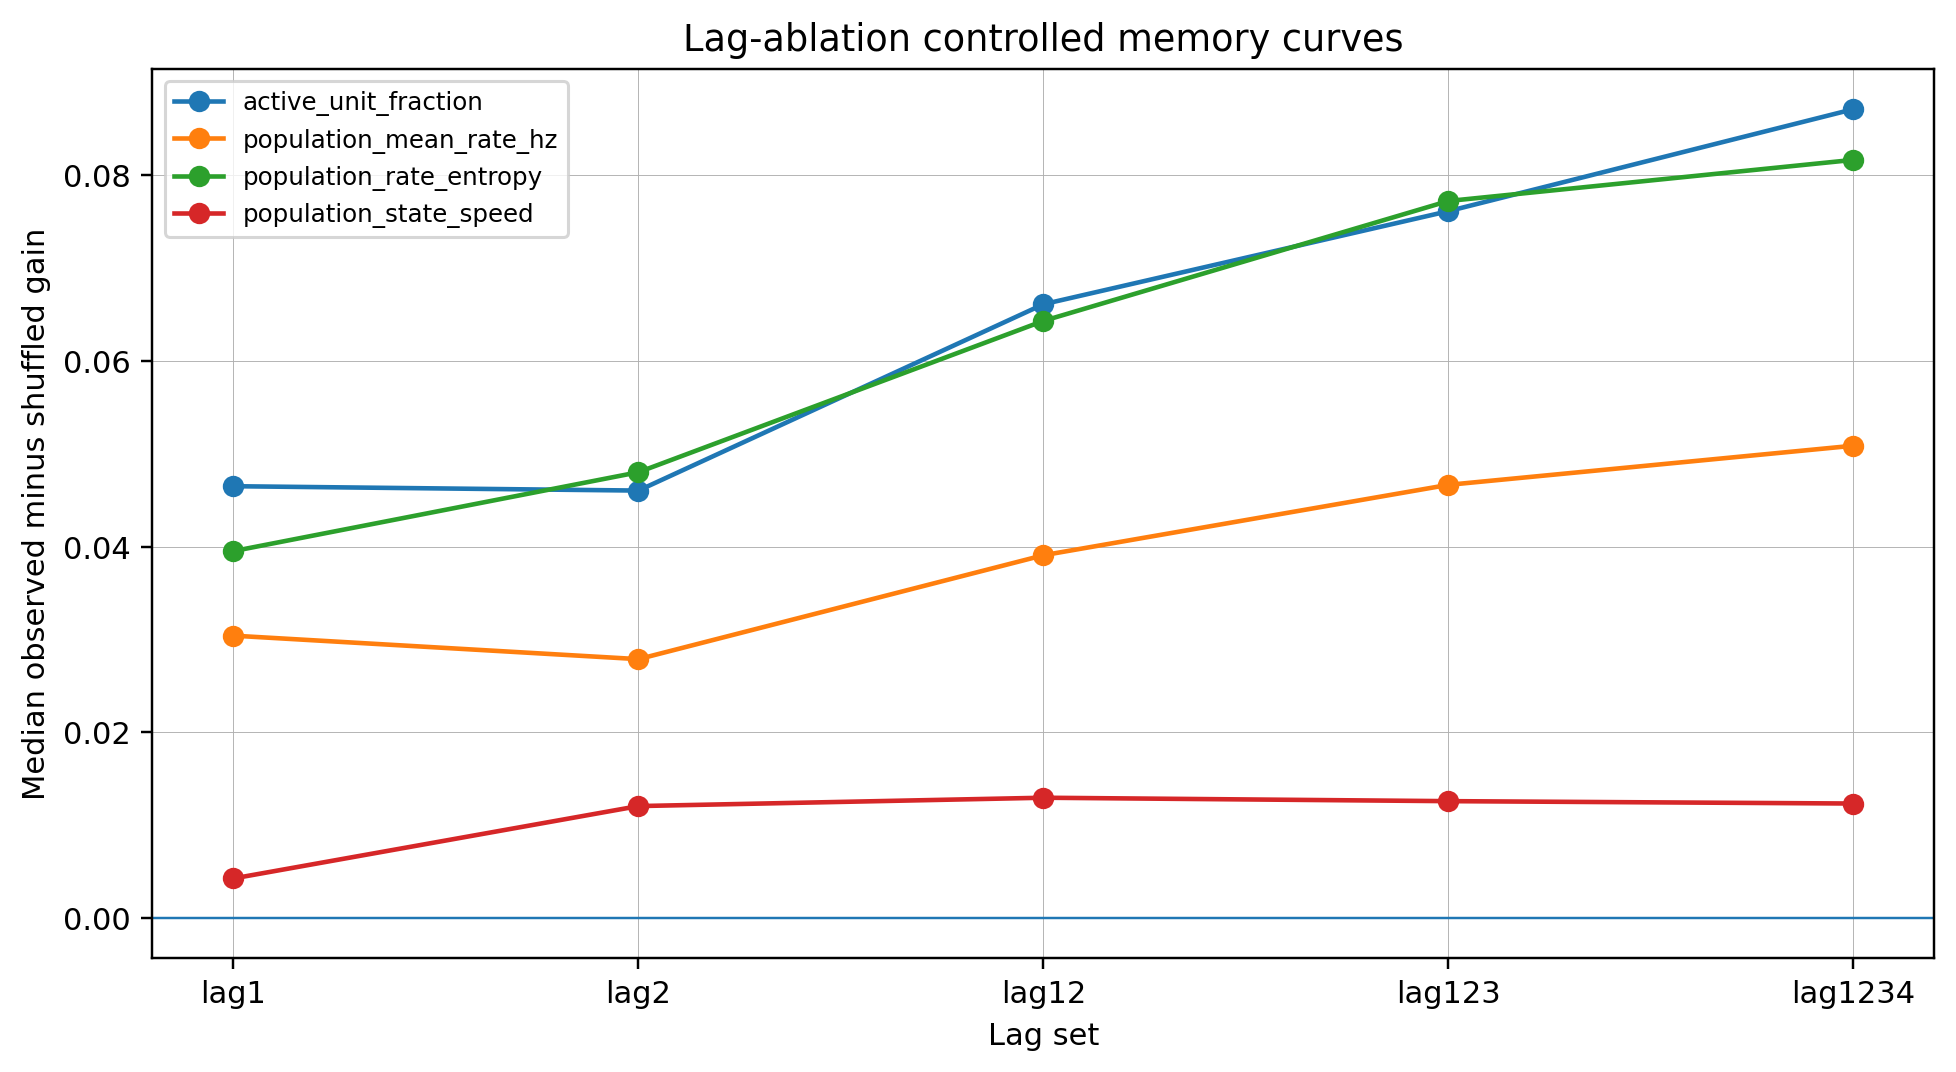
\includegraphics[width=0.85\linewidth]{results/figures/ablation/allen_spontaneous_v1/lag_ablation_controlled_memory_curves.png}
\caption{Lag-ablation curves. Active-unit fraction and population-rate entropy remain positive across lag choices, supporting the historical character of the controlled memory signal.}
\label{fig:lag-ablation}
\end{figure}

This result is stronger than the variance-scaling result. It indicates that the observed effect is not narrowly dependent on the initially selected lag pair.

\subsection{Descriptive ripeness separates state potential from memory-bearing organization}

A descriptive spontaneous neural ripeness index was computed from rank-normalized \(\Phi_{\rm neural}\), stability \(S\), controlled mean-rate memory, active-unit memory, and entropy memory. Penalties were applied for negative raw mean-rate memory gain or nonpositive controlled mean-rate memory gain. This index is descriptive rather than inferential.

The highest-ranked session-region state was:
\[
715093703 / \mathrm{VISl},
\]
with ripeness score \(0.777083\). At the region level, median ripeness ranked:
\[
\mathrm{CA1} > \mathrm{VISl} > \mathrm{LGd} > \mathrm{VISp}.
\]

\begin{table}[t]
\centering
\caption{Region-level descriptive ripeness summary. Ripeness does not simply reproduce \(\Phi_{\rm neural}\); CA1 and VISl rise when controlled organizational memory is included.}
\label{tab:ripeness}
\begin{tabular}{lrrrr}
\toprule
Region & Median ripeness & Mean ripeness & Median \(\Phi_{\rm neural}\) & Rank \\
\midrule
CA1 & 0.633333 & 0.581250 & -0.113984 & 1 \\
VISl & 0.591667 & 0.634028 & -0.067570 & 2 \\
LGd & 0.477083 & 0.485417 & 0.408474 & 3 \\
VISp & 0.381250 & 0.449306 & 0.131802 & 4 \\
\bottomrule
\end{tabular}
\end{table}

\begin{figure}[t]
\centering
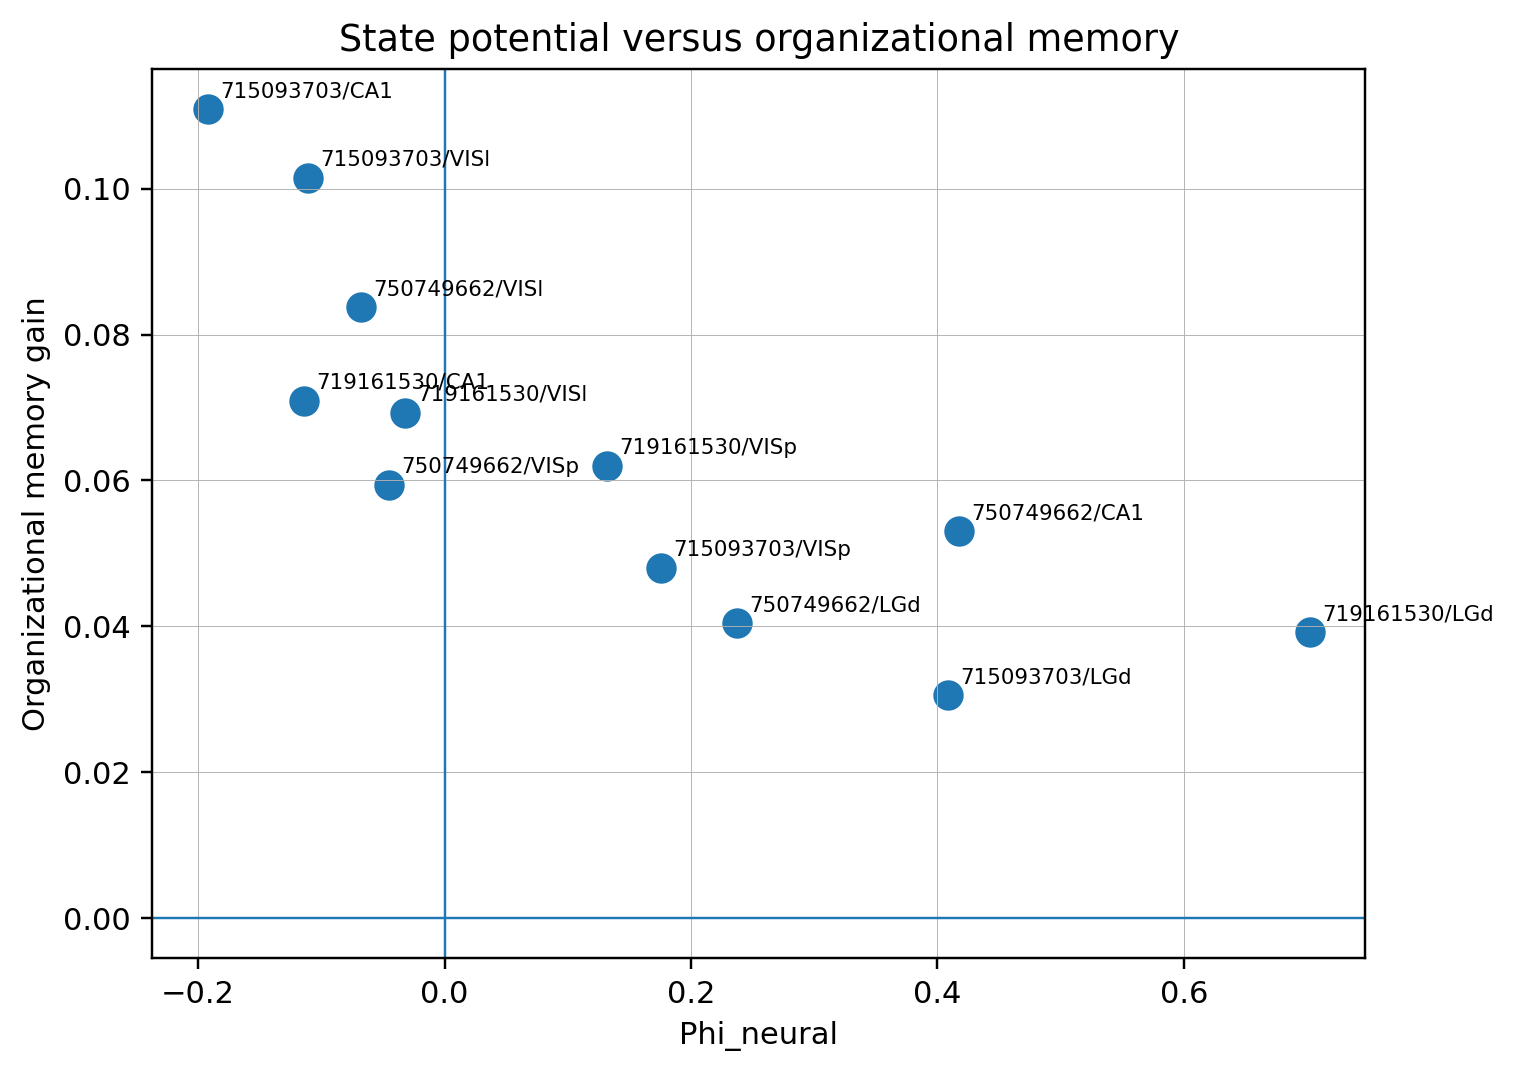
\includegraphics[width=0.78\linewidth]{results/figures/cross_session/allen_spontaneous_v1/spontaneous_neural_ripeness_phi_vs_memory.png}
\caption{Structural potential versus organizational memory. Descriptive ripeness separates high-\(\Phi_{\rm neural}\) structural states from states carrying strong controlled organizational memory.}
\label{fig:ripeness-phi-memory}
\end{figure}

The ripeness result is useful because it does not force LGd to the top. LGd remains structurally important, but CA1 and VISl become more ripened when controlled organizational memory is included. This distinction separates state potential from memory-carrying dynamics.

\section{Discussion}

This analysis supports a bounded conclusion: spontaneous neural population activity contains controlled organizational memory. Across three Allen Neuropixels sessions, aligned recent history improves prediction relative to shuffled-lag controls. The effect is strongest for variables describing population recruitment and distributional organization.

The result should not be interpreted as a generic claim that every region and every target exhibits positive raw memory gain. The third session contains a slightly negative raw VISp mean-rate gain. Nor should it be interpreted as a fixed regional hierarchy. LGd is the highest-\(\Phi_{\rm neural}\) region in two sessions, but CA1 is highest in the third. These exceptions are important because they sharpen the interpretation. The replicated component is not universal raw gain or universal LGd dominance. The replicated component is controlled historical contribution relative to shuffled-lag controls, especially in organizational targets.

The target-level result is the conceptual center of the study. Active-unit fraction and population-rate entropy rank above mean firing rate. This suggests that retained history is most visible in how the population organizes itself: which units participate and how activity is distributed across the population. This is consistent with broader evidence that spontaneous activity is structured, high-dimensional, and influenced by internal state and behavior \citep{Stringer2019Spontaneous,Akella2025LatentStates,Sederberg2024LatentDynamics}. It also aligns with information-theoretic approaches suggesting that organizational measures can reveal population structure not captured by classical variability measures \citep{DePaula2025StatisticalComplexity}.

The variance-scaling audit is a necessary constraint. Active-unit fraction remains the strongest raw controlled target, but it does not remain in the top two after residualizing variance and lag-1 autocorrelation. Entropy remains more stable under this audit. The manuscript therefore should not claim that recruitment memory is variance-independent. A more accurate statement is that recruitment and entropy dominate the raw controlled-memory ranking, while entropy is the cleaner target under variance/autocorrelation adjustment.

The lag-ablation audit provides stronger support for historical structure. Active-unit fraction and entropy remain positive across lag sets, and controlled gains increase as additional recent lags are included. This supports the operational non-Markovian interpretation: recent aligned history carries information about future population organization beyond shuffled-history controls.

The descriptive ripeness index should also be read cautiously. It is not a new biological law and not a consciousness measure. It is a state-ranking tool that combines structural HRSM position with controlled organizational memory. Its main value is conceptual: it separates structural potential from memory-carrying organization. LGd can be high-\(\Phi\) without being the ripest memory-bearing state, while CA1 and VISl can rise when organizational memory is included.

\section{Limitations}

The analysis is limited to three Allen Visual Coding Neuropixels sessions and four regions. The extraction scale was fixed at 20 units per region and 15 spontaneous presentations. The model class was ridge regression with lagged features. The shuffled-lag control is strong but not exhaustive. Other controls, including circular shifts, blockwise temporal shifts, region-label permutations, or alternative model classes, should be tested in future work.

The HRSM coordinates are operational proxies. They are useful for state-space analysis, but they should not be treated as direct physiological variables. The ripeness index is descriptive and should not be interpreted as consciousness, cognition, or subjective awareness.

The variance-scaling audit also limits the interpretation. Active-unit recruitment is partly entangled with variance and autocorrelation structure. Entropy is more robust under this audit, but additional datasets and controls are required before strong generalization.

\section{Conclusion}

A reduced HRSM state-space analysis of spontaneous Allen Neuropixels activity reveals a replicated controlled historical contribution to future population organization. Across three sessions, aligned recent history improves prediction relative to shuffled-lag controls. The strongest raw memory-sensitive targets are active-unit fraction and population-rate entropy. Variance and autocorrelation audits narrow the recruitment-specific claim, while entropy remains more stable. Lag-ablation tests support the historical character of the signal. Descriptive ripeness separates structural HRSM potential from memory-bearing organization. The resulting claim is deliberately bounded: spontaneous neural population activity carries controlled organizational memory.

\section*{Data availability}

No new animal data were generated. The analysis uses publicly available Allen Visual Coding Neuropixels data. Derived summaries, figures, and scripts are stored in the accompanying repository under the spontaneous Allen HRSM branch.

\section*{Code availability}

The analysis scripts are stored under \texttt{scripts/allen/}. The main outputs used in this manuscript are stored under \texttt{results/cross\_session/allen\_spontaneous\_v1/}, \texttt{results/real\_allen/}, and \texttt{results/ablation/allen\_spontaneous\_v1/}. A frozen reproducibility tag should be generated before submission.

\section*{Ethics statement}

This study reuses publicly released Allen Brain Observatory data. No new animal experiments were performed.

\section*{Competing interests}

The author declares no competing interests.

\section*{Author contributions}

S.A. designed the HRSM analysis framework, implemented the computational workflow, analyzed the Allen Neuropixels data, generated figures and robustness audits, and wrote the manuscript.

\section*{Acknowledgements}

The author acknowledges the Allen Institute for publicly releasing the Visual Coding Neuropixels dataset and associated documentation.

\bibliographystyle{plainnat}
\bibliography{paper/references}

\appendix

\section{Supplementary result inventory}

The following outputs support the main manuscript:

\begin{itemize}
    \item \texttt{cross\_session\_spontaneous\_session\_summary.csv}
    \item \texttt{cross\_session\_spontaneous\_target\_synthesis.csv}
    \item \texttt{cross\_session\_spontaneous\_replication\_flags.csv}
    \item \texttt{variance\_scaling\_target\_residual\_summary.csv}
    \item \texttt{variance\_scaling\_correlation\_summary.csv}
    \item \texttt{lag\_ablation\_cross\_session\_target\_summary.csv}
    \item \texttt{spontaneous\_neural\_ripeness\_index.csv}
\end{itemize}

\section{Supplementary robustness flags}

The three-session synthesis produced the following primary flags:

\begin{verbatim}
all_sessions_memory_gain_positive = False
all_sessions_above_shuffle = True
orthogonality_numeric_precision = True
top_targets_are_recruitment_and_entropy = True
LGd_best_phi_in_each_session = False
\end{verbatim}

The variance-scaling audit produced:

\begin{verbatim}
top_two_raw_are_recruitment_and_entropy = True
top_two_residual_are_recruitment_and_entropy = False
overall_variance_correlation_not_extreme = True
\end{verbatim}

The lag-ablation audit produced:

\begin{verbatim}
lag12_top_two_are_recruitment_and_entropy = True
recruitment_entropy_positive_all_lagsets = True
\end{verbatim}

The ripeness audit produced:

\begin{verbatim}
all_ripeness_scores_finite = True
top_state_has_positive_controlled_memory = True
top_region_not_forced_to_LGd = True
organizational_memory_positive_in_top_half = True
\end{verbatim}

\end{document}
